\chapter{深度伪造的研究工具与检测手段的分类}
\label{chap:3}

本章节探讨深度伪造的研究工具与检测手段的分类,首先会根据 Thanh Thi Nguyen 等人 \cite{https://doi.org/10.48550/arxiv.1909.11573} 所进行的研究工作的简述,在他们的工作总结中将其工具分为两大类,也就是图像检测与人脸视频检测,并有着详细的整理,此外根据 Li XR 等人近期对深度伪造与检测的汇整工作\cite{2021496} 也有着详尽的说明,本作业除了针对究工具与检测手段等研究者们的近来工作将其汇整于此章。

\begin{figure}[htb]
\centering 
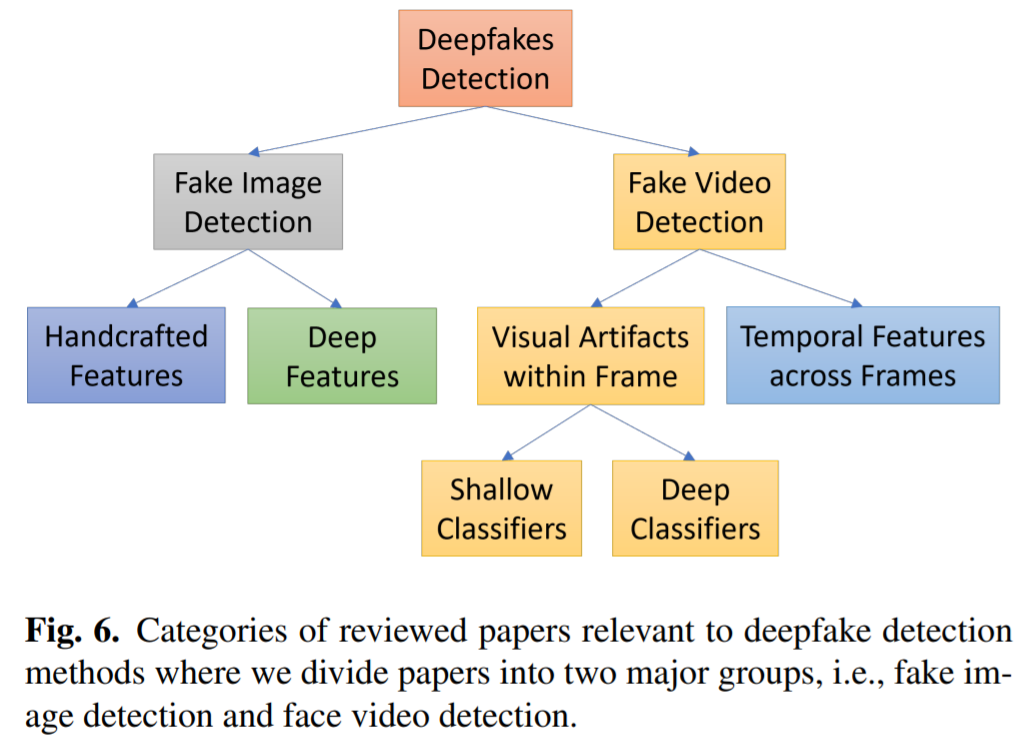
\includegraphics[width=0.90\textwidth]{img/ch3m1.png} 
\caption{从由 Thanh Thi Nguyen 等人 \cite{https://doi.org/10.48550/arxiv.1909.11573} 将深度伪造的伪造分为两大类}
\label{Test}
\end{figure}


\section{深度伪造的图像检测与人脸视频检测整理}

根据由 Thanh Thi Nguyen 等人 \cite{https://doi.org/10.48550/arxiv.1909.11573}的在深度伪造的工作中所整理的分类整理的过程中将其分为了图像检测与人脸视频检测。同时该工作也有将其深度伪造的检测手段进行总结,本作业根据原总结工作再汇整为深度伪造检测手段整理两表,两表之中总共有 24 种检测手段,这当中又因该工作所进行的分类,而分为三部分,其一为针对图像的检测,列于表二,共有 9 种手段,其二为影像的检测手段,其列于表一,共有 13 种手段,其三为图像检测与人脸视频检测皆可的检测,只有两种手段,并与表二图像检测并列。



%\begin{table}[ht]
%  \caption{test}
%  \label{Tab:bookRWCal}
%  \centering
%  \begin{tabular}{lp{3cm}p{3cm}p{3cm}}
%  \toprule
%  \textbf{著作类别} &\textbf{A级出版社} &\textbf{B级出版社}&\textbf{C级出版社}\\
%  \midrule
%  学术专著         &第一作者3分/万字,其他作者 2分/万字	&第一作者3分/万字,其他作者 2分/万字	&第一作者3分/万字,其他作者 2分/万字\\
%  \bottomrule
%  \end{tabular}
%\end{table}

\begin{table}[ht]
  \caption{深度伪造检测手段整理}
  \label{Tab:bookRWCal}
  \centering
  %\begin{tabular}{lp{3cm}p{2cm}p{2cm}}
  \begin{tabular}{p{3cm}p{3cm}p{3cm}p{3cm}}
  \toprule
  \textbf{方法} &\textbf{技術} &\textbf{检测种类}&\textbf{备注}\\
  \midrule
 Eye blinking & LRCN & Videos & Yuezun Li 等人\\
 Intra-frame and temporal inconsistencies & CNN and LSTM & Videos & David Guera 等人\\
 Using face warping artifacts & VGG16, ResNet models & Videos & Yuezun Li 等人\\
 MesoNet & CNN & Videos & Darius Afchar 等人\\
 Eye, teach and facial texture & Logistic regression and neural network(NN) & Videos & Falko Matern 等人\\
 Spatio-temporal features with RCN & RCN & Videos & Ekraam Sabir 等人\\
 Spatio-temporal features with LSTM & Convolutional bidirectional recurrent LSTM network & Videos & Akash Chintha 等人\\
 Analysis of PRNU & PRNU & Videos & Marissa Koopman 等人\\
 Phoneme-viseme mismatches & CNN & Videos & Shruti Agarwal 等人\\
 Using attributionbased confidence (ABC) metric & ResNet50 model, pre-trained on VGGFace2 & Videos & Steven Fernandes 等人\\
 Using appearance and behaviour & Rules based on facial and behavioural features & Videos &  Shruti Agarwal 等人\\
 FakeCatcher & CNN & Videos & Umur Aybars Ciftci 等人\\
 Emotion audiovisual affective cues & Siamese network & Videos & Trisha Mittal 等人\\
  \bottomrule
  \end{tabular}
\end{table}

\begin{table}[ht]
  \caption{深度伪造检测手段整理(续)}
  \label{Tab:bookRWCal}
  \centering
  %\begin{tabular}{lp{3cm}p{2cm}p{2cm}}
  \begin{tabular}{p{3cm}p{3cm}p{3cm}p{3cm}}
  \toprule
  \textbf{方法} &\textbf{技術} &\textbf{检测种类}&\textbf{备注}\\
  \midrule
 Head poses & SVM & Videos and Images & Xin Yang 等人\\
 Capsule-forensics & Capsule networks & Videos and Images & Huy H Nguyen 等人\\
 Preprocessing combined with deep network & DCGAN, WGAN-GP and PGGAN. & Images & Xinsheng Xuan 等人\\
 Analyzing convolutional traces & KNN, SVM, and linear discriminant analysis (LDA) & Images &  Luca Guarnera 等人\\
 Bag of words and shallow classifiers & SVM, RF, MLP & Images & Ying Zhang 等人\\
 Pairwise learning & CNN concatenated to CFFN & Images & Chih-Chung Hsu 等人\\
 Defenses against adversarial perturbations in deepfakes & VGG and ResNet & Images &  Apurva Gandhi 等人\\
 Face X-ray & CNN & Images & Chih-Chung Hsu 等人\\
 Using common artifacts of CNN-generated images & ResNet-50 pre-trained with ImageNet & Images & Sheng-Yu Wang 等人\\
 Using convolutional traces on GAN-based images & KNN, SVM, and LDA & Images & Luca Guarnera 等人\\
 Using deep features extracted by CNN & A new CNN model, namely SCnet & Images & Zhiqing Guo 等人\\
  \bottomrule
  \end{tabular}
\end{table}

\section{过往传统的检测手段}

过往的方式多为根据图像的特征来进行,其手段大多为信号的处理方式,且多数依赖某些特有的窜改证据,同时根据图像本身自有的频域特征与统计特征来进行分类,这些方式如噪音分析、设备指纹、光照、图像品质、处理复制移动、拼接、移除等问题,其实际工作比如 De Carvalho TJ 等人 \cite{de2013exposing},提出了一种伪造检测方法,该方法利用图像照明颜色的细微不一致,其方法是基于机器学习的,并且需要最少的用户交互。该技术适用于包含两个或更多人的图像,并且不需要专家交互来做出篡改决定,为了实现这一点,研究者将来自基于物理和统计的光源估计器的信息整合到类似材料的图像区域上。从这些光源估计中,该研究者提取基于纹理和边缘的特征,然后将其提供给机器学习方法以进行自动决策。使用 SVM 元融合分类器的分类性能是有希望的。它在由 200 张图像组成的新基准数据集上产生 86\% 的检测率,在从 Internet 收集的 50 张图像上产生 83\% 的检测率。

\begin{figure}[htb]
\centering 
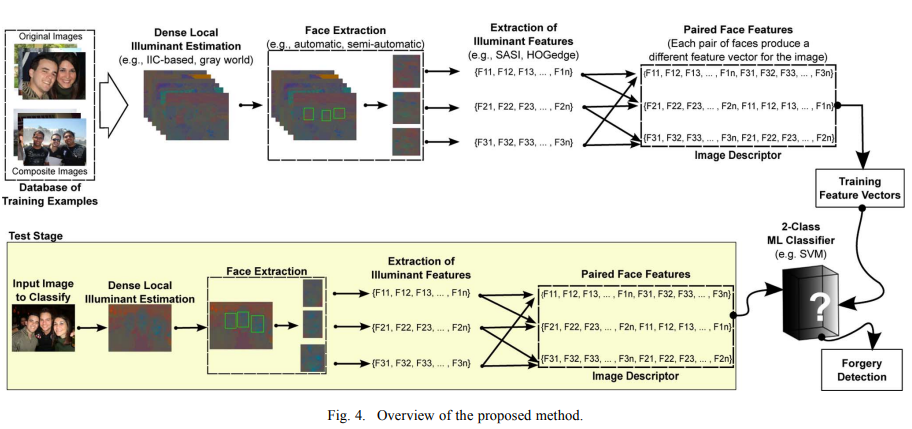
\includegraphics[width=0.90\textwidth]{img/ch3m2.png} 
\caption{De Carvalho TJ 等人 \cite{de2013exposing}}
\label{Test}
\end{figure}

另外  Amerini I 等人 \cite{amerini2011sift} 则探究图像是否被伪造的检测问题;特别是,图像的一个区域被复制然后粘贴到另一个区域用以创建复制或取消一些尴尬的东西的情况。通常来说为了使图像补丁适应新的上下文,需要进行几何变换。为了检测这种修改,提出了一种基于尺度不变特征变换(SIFT)的新方法。这种方法使研究者既可以了解是否发生了复制移动攻击,还可以恢复用于执行克隆的几何变换。广泛的实验结果证实了该技术能够精确地个体化改变区域,此外,还能够以高可靠性估计几何变换参数。该方法还处理多重复制。

同理可推,其深度伪造的影像的本质,实质上也是一连串的图像伪造的工作合成后所完成的结果,也因为如此,此类检测方式与手段就能使用到深度伪造的检测工作上。而 Lukáš J \cite{lukavs2006detecting} 等人提出了一种检测数字图像中的伪造品的新方法,其方法基于检测图像中各个区域中相机模式噪声的存在,这是成像传感器的独特随机特性。而伪造区域被确定为缺少图案噪声的区域。噪声的存在是使用相关性确定的,如在扩频水印的检测中。研究者们提出了两种方法在第一个中,用户选择一个区域进行完整性验证。第二种方法试图在不假设任何先验知识的情况下自动确定伪造区域。这些方法在真实伪造的例子和非伪造图像上都进行了测试,其研究者还研究了应用于伪造图像的进一步图像处理,例如有损压缩或过滤,如何影响验证图像完整性的能力。

\begin{figure}[htb]
\centering 
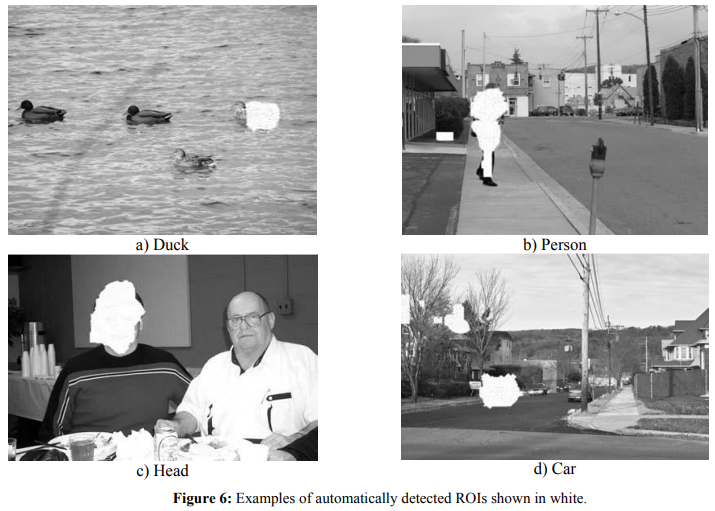
\includegraphics[width=0.90\textwidth]{img/ch3m3.png} 
\caption{Lukáš J 等人 \cite{lukavs2006detecting}}
\label{Test}
\end{figure}

Chierchia G 等人 \cite{chierchia2011prnu} 引入了光响应非均匀性 (PRNU) 作为检测图像伪造的强大工具,尽管它在许多情况下都有效,但所提出的方法无法检测到小的操作。在这项工作中,研究者基于图像的初步分割提出了中描述的检测算法的修改版本,这保证了对小尺寸加法伪造品的更好检测性能。而 Fridrich J 等人 \cite{fridrich2012rich} 则提出一种新的通用策略,用于为数字图像构建隐写检测器,该过程首先组装一个丰富的噪声分量模型,作为由使用线性和非线性高通滤波器获得的量化图像噪声残差的相邻样本的联合分布形成的许多不同子模型的联合。与以前的方法相比,研究者使模型组装成为训练过程的一部分,该过程由从相应的覆盖和隐秘源中抽取的样本驱动。集成分类器用于组装模型以及最终的隐写分析器,因为它们的计算复杂度低并且能够有效地处理高维特征空间和大型训练集。该研究在三种隐写算法上演示了所提出的框架,这些演算法旨在隐藏空间域中表示的图像中的消息:HUGO、Luo 的边缘自适应算法和优化编码的三元 ±1 嵌入。对于每种算法,研究者应用一种简单的子模型选择技术来提高每个模型维度的检测精度,并展示检测如何随着丰富模型的复杂性增加而饱和。通过观察不同子模型如何参与检测之间的差异,揭示了嵌入和检测之间有趣的相互作用。围绕丰富的图像模型构建的隐写分析与集成分类器相结合,是为广泛的隐写方案自动化隐写分析的一个有前途的方向。另外 Wang W 等人 \cite{wang2014exploring} 则专注于局部图像篡改检测。对于 JPEG 图像,其 DCT 系数的概率分布会受到篡改操作的干扰,篡改区域和未改动区域分布不同,是定位篡改的重要线索。基于未量化的ac DCT系数的拉普拉斯分布假设,可以估计这两个分布以及被篡改区域的大小,从而得到每个DCT块被篡改的概率,当研究者考虑常见篡改区域的先验知识时,可以获得更准确的定位结果,其研究者还设计了三种可以区分真实篡改区域和虚假区域的特征,以减少误报。对于以无损压缩格式保存的篡改图像,而研究者还提出了一种专门的方法,该方法利用高频DCT系数的量化噪声来提高篡改定位性能。在大规模数据库上的大量实验证明了该研究提出的方法的有效性,并证明其方法适用于定位不同尺度的篡改区域。

此外還對 JPEG 压缩的图像中添加噪声來進行檢測的研究,比如 Nataraj L 等人 \cite{nataraj2009adding} 认为影响大多数图像大小调整检测算法的一个常见问题是它们容易受到 JPEG 压缩的影响,这是因为 JPEG 引入了周期性伪影,因为它适用于 8×8 块。其研究者提出了一种新颖但反直觉的技术,通过添加高斯噪声来“去噪”JPEG 图像。其研究者将适量的高斯噪声添加到调整大小和 JPEG 压缩的图像中,以便抑制由于 JPEG 压缩而导致的周期性,而由于调整大小而导致的周期性得以保留,受控的高斯噪声添加比中值滤波和基于加权平均的滤波更有效地抑制 JPEG 引起的周期性。

\begin{figure}[htb]
\centering 
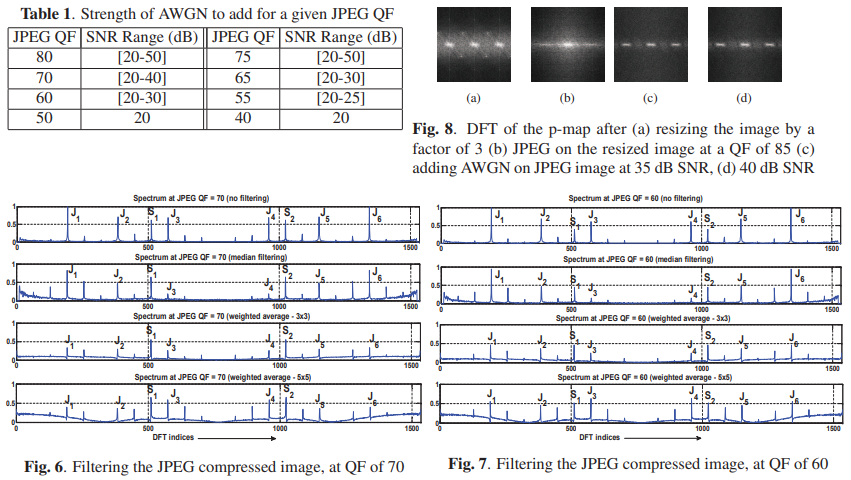
\includegraphics[width=0.90\textwidth]{img/ch3m4.png} 
\caption{Nataraj L 等人 \cite{nataraj2009adding}}
\label{Test}
\end{figure}

同时 Bianchi T 等人 \cite{bianchi2011improved} 提出了一种统计测试来区分 JPEG 图像中的原始区域和伪造区域,假设前者是双重压缩的,而后者是单次压缩的。提出了单压缩和双压缩区域 DCT 系数的新概率模型,以及双压缩情况下估计主量化因子的可靠方法,基于这样的模型,推导出每个 DCT 块被伪造的概率,其实验结果证明了相对于先前提出的方法更好的区分行为。

另外有些研究者则运用局部噪音方差分析的特性来拼接痕迹 Pan X 等人 \cite{pan2012exposing} 所提出的研究是基于来自不同来源的图像往往具有由传感器或后处理步骤引入的不同数量的噪声,研究者描述了一种通过检测局部噪声方差的不一致性来暴露图像拼接的有效方法,其方法基于以下观察估计局部噪声方差:带通滤波域中自然图像的峰度值倾向于集中在一个恒定值附近,并通过使用积分图像来加速。最后基于通过图像拼接生成的几组伪造图像证明了我们方法的有效性和鲁棒性。

而 Ferrara P \cite{6210378} 等人则是运用 色彩过滤矩阵 (Color Filter Array; CFA) 模型来找出修改过的地方,该研究提出了一种能够区分数码相机捕获的图像中的原始区域和伪造区域的取证工具,研究者假设图像是使用滤色器阵列获取的,并且由于去马赛克算法,篡改会消除伪影,其所提出的方法是基于一个新的特征来测量局部水平的去马赛克伪影的存在,以及一个新的统计模型,允许推导出每个 2 × 2 图像块的篡改概率,而无需先验地知道伪造的位置。最后在配备不同去马赛克算法的不同相机上的实验结果证明了理论模型的有效性和方案的有效性。

\begin{figure}[htb]
\centering 
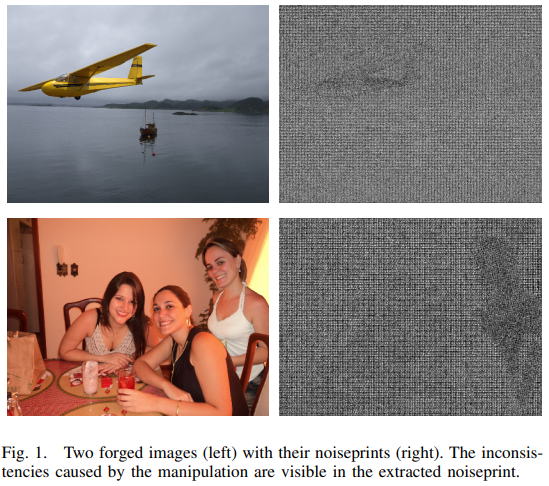
\includegraphics[width=0.90\textwidth]{img/ch3m5.png} 
\caption{Cozzolino D 等人 \cite{cozzolino2019noiseprint}}
\label{Test}
\end{figure}

由于近年来人工智能领域的进步,当中的机器学习下的深度学习方法逐渐导入检测手段中,其卷积神经网络、生成对抗网路与 Transformer 等模型,在该领域的应对皆超越了过往的纪录,而且成功率大大的提升,相较上述过往图像特征的检测方式,前者的鲁棒性更好。Cozzolino D 等人 \cite{cozzolino2019noiseprint} 则认为数字图像的取证分析在很大程度上依赖于在获取的图像上留下的相机内和相机外过程的痕迹,这样的痕迹代表了一种相机指纹,若能够恢复它们,通过抑制高级场景内容和其他干扰,可以轻松完成多项取证任务。一个值得注意的例子是 PRNU 模式,它可以被视为设备指纹,在多媒体取证中受到了极大的关注。该研究提出了一种提取相机模型指纹的方法,称为噪声指纹,其中场景内容在很大程度上被抑制,与模型相关的伪影得到增强。这是通过连体网络获得的,该网络使用来自相同(标签 +1)或不同(标签 -1)相机的成对图像块进行训练。尽管噪声印记可用于多种取证任务,但这里我们专注于图像伪造定位,而在广泛使用的几个数据集上的实验表明,基于噪声印记的方法可以提供最先进的性能。Zhou P 等人 \cite{zhou2018learning}认为图像操作检测不同于传统的语义对象检测,因为它更关注篡改伪影而不是图像内容,这表明需要学习更丰富的特征,研究者提出了一个双流 Faster R-CNN 网络并对其进行端到端训练,以检测给定操纵图像的篡改区域。两个流之一是 RGB 流,其目的是从 RGB 图像输入中提取特征,以发现篡改伪影,如强对比度差异、不自然的篡改边界等。另一种是噪声流,它利用从隐写分析丰富的模型过滤层中提取的噪声特征来发现真实区域和篡改区域之间的噪声不一致。然后,研究者通过双线性池化层融合来自两个流的特征,以进一步结合这两种模式的空间共现。对四个标准图像处理数据集的实验表明,其双流框架优于每个单独的流,并且与具有调整大小和压缩鲁棒性的替代方法相比,还实现了最先进的性能。

Rao Y 等人 \cite{rao2016deep} 提出了一种基于深度学习技术的新图像伪造检测方法,该方法利用卷积神经网络 (CNN) 从输入的 RGB 彩色图像中自动学习层次表示,所提出的 CNN 专为图像拼接和复制移动检测应用而设计,其网络第一层的权重不是随机策略,而是使用空间丰富模型 (SRM) 中残差图计算中使用的基本高通滤波器集进行初始化,作为正则化器,可以有效地抑制图像内容并捕获由篡改操作引入的细微伪影,将预训练的 CNN 作为补丁描述符从测试图像中提取密集特征,然后探索特征融合技术以获得 SVM 分类的最终判别特征。在几个公共数据集上的实验结果表明,所提出的基于 CNN 的模型优于一些最先进的方法。Liu B 等人 \cite{liu2018deep} 提出了一种新颖的深度融合网络,通过跟踪其边界来定位篡改区域,首先训练了一组称为 Base-Net 的深度卷积神经网络来分别响应某种类型的拼接伪造。然后,选择 Base-Net 的一些层并组合为深度融合神经网络(Fusion-Net),经过极少量的图片微调后,Fusion-Net 能够辨别图像块是否是从不同来源合成的。在基准数据集上的实验表明,该研究方法在各种情况下都是有效的,并且优于最先进的方法。Huh M 等人  \cite{huh2018fighting} 认为照片编辑和操作工具的进步使得创建假图像变得更加容易,突出了对更好的视觉取证算法的需求,然而,由于缺乏被操纵的视觉内容的良好数据集,学习从标记的训练数据中检测操纵是困难的,该研究介绍了一种自我监督方法,用于学习仅使用未标记数据来检测视觉操作。给定大量带有自动记录的 EXIF 元数据的真实照片,研究者训练一个模型来确定图像是否是自洽的——也就是说,它的内容是否可以由单个成像管道产生。研究者将这种自我监督学习方法应用于定位拼接图像内容的任务。其取证模型在许多基准上都取得了最先进的结果,尽管在没有实际操作示例的情况下进行了训练,也没有对特定的检测线索进行建模。除了手工制作的基准之外,研究者还展示了在 Reddit 和 The Onion 上发现假货以及检测计算机生成的拼接的有希望的结果。Cun X 等人 \cite{cun2018image} 解决了图像拼接定位的问题:给定一张输入图像,定位从另一张图像中剪下的拼接区域,并将其制定为分类任务,但关键的是,我们不是通过局部补丁对拼接区域进行分类,而是利用整个图像和局部补丁的特征来对补丁进行分类。而研究者们称这种结构为 Semi-Global Network,其方法利用了拼接区域不仅应与局部特征(拼接边缘)高度相关,还应与整个图像的全局特征(语义信息、照明等)高度相关的观察结果。此外,该研究首先将全连接条件随机场作为图像拼接中的后处理技术,以提高输入图像和网络输出之间的一致性。

Cozzolino D 等人 \cite{cozzolino2017recasting} 基于图像噪声残差的局部描述符已被证明对于许多取证应用非常有效,例如伪造检测和定位,尽管如此,在计算机视觉领域取得可喜成果的推动下,研究界的重点现在正在转向深度学习。该研究展示了一类基于残差的描述符实际上可以被视为一个简单的约束卷积神经网络(CNN)。通过放松约束,并在相对较小的训练集上微调网络,其成果相对于传统检测器获得了显著的性能提升。

\begin{figure}[htb]
\centering 
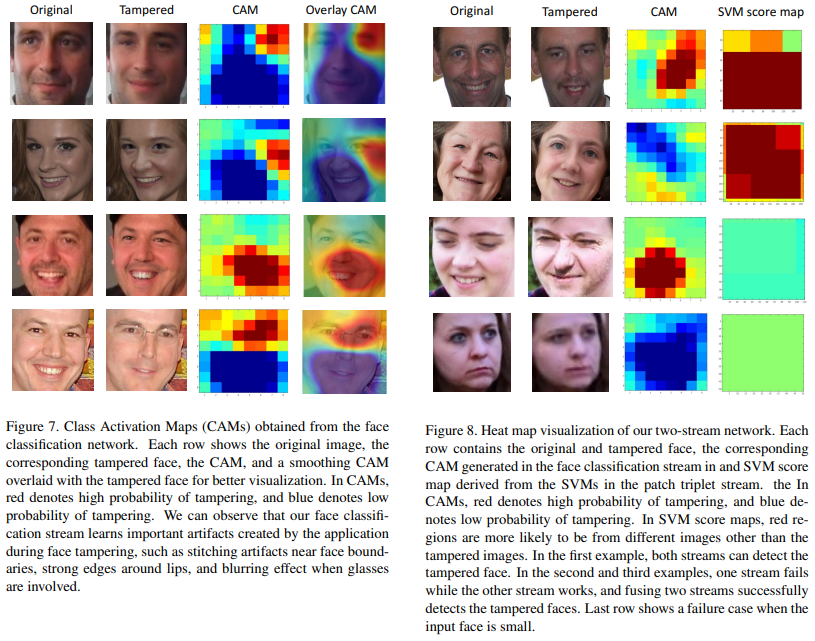
\includegraphics[width=0.90\textwidth]{img/ch3m6.png} 
\caption{Zhou P 等人 \cite{zhou2017two}}
\label{Test}
\end{figure}

Chen C 等人 \cite{chen2018focus} 认为随着通过社交媒体渠道传播的错误信息的兴起,以及图像处理工具的自动化和真实性的提高,图像取证成为一个越来越重要的问题,经典的图像取证方法利用低级线索,例如元数据、传感器噪声指纹等,当图像在上传到 Facebook 等时重新编码时很容易被愚弄。这需要使用更高级别的物理和语义线索,这些线索曾经在野外难以可靠地估计,但由于计算机视觉的能力越来越强,它们变得更加有效。特别是,该研究的检测由图像的人工模糊引入的操作,这会在图像强度和各种线索之间产生不一致的光度关系。在一个新的模糊操作数据集中,研究者在最具挑战性的情况下实现了 98\% 的准确率,其中模糊在几何上是正确的并且与场景的一致 物理安排。这种操作现在很容易生成,例如,通过具有硬件来测量深度的智能手机相机,例如。 iPhone7Plus 的“人像模式”。最后还在挑战数据集上展示了良好的性能,该数据集评估了代表“野外”条件的图像中更广泛的操作。

Zhou P 等人 \cite{zhou2017two} 则根据 Szegedy C 等人 \cite{szegedy2015going}所提出的基础上,做出了一种用于人脸篡改检测的双流网络,其训练 GoogLeNet 以检测人脸分类流中的篡改伪影,并训练基于补丁的三元组网络以利用捕获局部噪声残差和相机特征的特征作为第二个流。此外,研究者使用两个不同的在线人脸交换应用程序来创建一个新的数据集,该数据集由 2010 个篡改图像组成,每个图像都包含一个被篡改的人脸。最后在新收集的数据集上评估提出的双流网络。实验结果证明了其方法的有效性。

\section{人类的生理特征的检测手段}

深度伪造的影像往往会忽视人类正常活动的生理特征,因而无法在整体的状况下与真实人类的行动与反应一致,所以根据人类的生理信号特征也进入了研究者们关注的部分。 Yang X 等人 \cite{yang2019exposing} 所提出的方法是基于观察到 DeepFakes 是通过将合成的人脸区域拼接到原始图像中来创建的,并且在这样做的过程中,当从人脸图像估计 3D 头部姿势时可以发现错误。研究者进行实验来证明这种现象,并进一步开发基于这种线索的分类方法。使用基于此线索的特征,使用一组真实面部图像和 DeepFakes 评估 SVM 分类器。同样也是 Yang X 等人 \cite{yang2019exposing} 发现生成对抗网络(GAN)最近导致了高度逼真的图像合成结果。在这项工作中,研究者描述了一种使用面部标志点的位置来展示 GAN 合成图像的新方法。其方法是基于观察到,由于缺乏全局约束,GAN 模型生成的面部部件配置与真实面部不同。研究者进行了演示这种现象的实验,并表明使用面部标志点的位置训练的 SVM 分类器足以为 GAN 合成的面部实现良好的分类性能。

\begin{figure}[htb]
\centering 
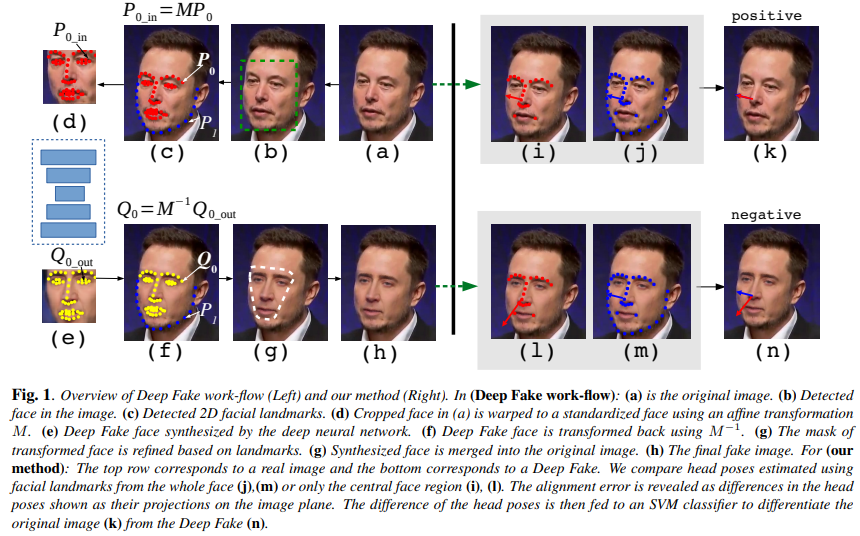
\includegraphics[width=0.90\textwidth]{img/ch3m7.png} 
\caption{Yang X 等人 \cite{yang2019exposing}}
\label{Test}
\end{figure}

另外 Li Y 等人 \cite{liy2018exposingaicreated} 认为深度生成网络的新发展显著提高了生成逼真的假人脸视频的质量和效率。在这项工作中,研究者描述了一种新方法来暴露由深度神经网络模型生成的假人脸视频,其方法基于检测视频中的眨眼,这是一种生理信号,在合成的假视频中没有很好地呈现。该方法在眨眼检测数据集的基准上进行了评估,并在检测使用基于 DNN 的软件 DeepFake 生成的视频方面表现出良好的性能。

而 Ciftci UA 等人 \cite{ciftci2020fakecatcher} 提出了一种检测肖像视频中合成内容的新方法,作为针对深度伪造威胁的预防性解决方案。换句话说,该研究引入了一个深度伪造检测器,研究观察到,盲目地利用深度学习的检测器无法有效捕捉虚假内容,因为生成模型会产生非常逼真的结果。其研究者的关键断言是,隐藏在肖像视频中的生物信号可以用作真实性的隐含描述符,因为它们既不会在空间上也不会在时间上保留在虚假内容中。为了证明和利用这一断言,该研究首先对成对分离问题进行了几次信号转换,达到了 99.39\% 的准确率。其次,通过分析建议的信号转换和相应的特征集,利用这些发现为虚假内容制定通用分类器。第三,生成新的信号图并使用 CNN 来改进我们用于检测合成内容的传统分类器。最后,发布了一个“在野外”的假肖像视频数据集,而后在评估过程中收集了该数据集。研究在几个数据集上评估 FakeCatcher,分别在人脸取证、人脸取证++、CelebDF 和研究本身新的 Deep Fakes 数据集上获得 96\%、94.65\%、91.50\% 和 91.07\% 的准确率。该研究还分析了来自不同面部区域的信号,在图像失真下,具有不同的片段持续时间,来自不同的生成器,针对看不见的数据集,以及在几种降维技术下。

同时 Fernandes S 等人 \cite{fernandes2019predicting} 获得了原始视频的心率并训练了最先进的神经常微分方程 (Neural-ODE) 模型。然后,研究者使用商业软件制作了 deepfake 视频,其十个原始视频获得的平均损失为 0.010927,十个捐赠视频为 0.010041,经过训练的 Neural-ODE 能够预测我们使用商业软件生成的 10 个 deepfake 视频和 deepfakeTIMI 数据库的 320 个 deepfake 视频的 heart rate,据该研究者所知,这是首次尝试在原始视频上训练 Neural-ODE 来预测假视频的 heart rate。


\section{图像伪造后留下痕迹的检测手段}

\begin{figure}[htb]
\centering 
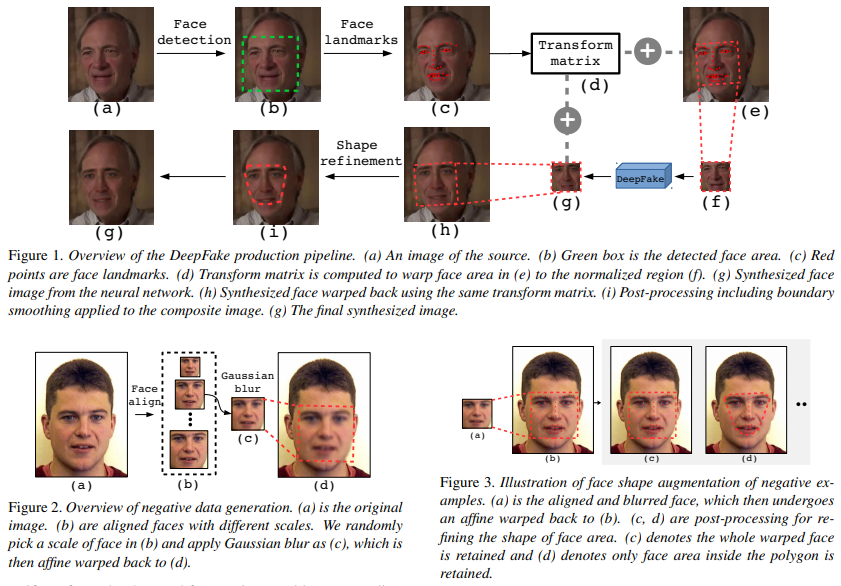
\includegraphics[width=0.90\textwidth]{img/ch3m8.png} 
\caption{ Li Y 等人 \cite{li2018exposing} }
\label{Test}
\end{figure}

其深度伪造的成果受限于过往深度学习的技术发展,用此技术所生成的人类脸部替换或者是伪造的细节皆没有很理想,因此不少研究者为此投入这个部分,而 Li Y 等人 \cite{li2018exposing} 描述了一种新的基于深度学习的方法,可以有效地将 AI 生成的假视频(以下称为 {\em DeepFake} 视频)与真实视频区分开来。其方法基于当前 DeepFake 算法只能生成分辨率有限的图像的观察结果,这些图像需要进一步变形以匹配源视频中的原始人脸,这种变换在生成的 DeepFake 视频中留下了独特的伪影,我们证明它们可以被卷积神经网络 (CNN) 有效地捕获,与以前使用大量真实和 DeepFake 生成的图像来训练 CNN 分类器的方法相比,该方法不需要 DeepFake 生成的图像作为负训练示例,因为研究将仿射面部扭曲中的伪影作为区分真假的显著特征图片。其研究方法的优点有两个:(1)可以直接对图像使用简单的图像处理操作来模拟这种伪影,使其成为反例。由于训练 DeepFake 模型生成负样本既费时又需要资源,因此该研究的方法在训练数据收集方面节省了大量时间和资源; (2) 由于此类伪影普遍存在于来自不同来源的 DeepFake 视频中,因此该研究的方法与其他方法相比更加稳健,研究的方法在两组 DeepFake 视频数据集上进行了评估,以了解其在实践中的有效性。

最后 Li Y 等人 \cite{li2018exposing} 则是运用了 He K 等人 \cite{he2016deep}所做的一个残差学习框架,以简化比以前使用的网络更深的网络的训练,该研究明确地将层重新定义为参考层输入的学习残差函数,而不是学习未参考的函数。其提供了全面的经验证据,表明这些残差网络更容易优化,并且可以从显著增加的深度中获得准确性。在 ImageNet 数据集上,研究者评估深度高达 152 层的残差网络——比 VGG 网络深 8 倍,但仍然具有较低的复杂度,这些残差网络的集合在 ImageNet 测试集上实现了 3.57\% 的误差。该结果在 ILSVRC 2015 分类任务中获得第一名。我们还对具有 100 层和 1000 层的 CIFAR-10 进行了分析。表示的深度对于许多视觉识别任务至关重要,其研究在 COCO 对象检测数据集上获得了 28\% 的相对改进,深度残差网络是该研究提交 ILSVRC 和 COCO 2015 比赛的基础,研究者还在 ImageNet 检测、ImageNet 定位、COCO 检测和 COCO 分割任务中获得了第一名,也就是所谓的 ResNet 框架。

另外 Matern F 等人 \cite{matern2019exploiting} 回顾了当前的面部编辑方法和来自其处理管道的几个特征工件。其研究还表明,相对简单的视觉伪影在暴露此类操作方面已经非常有效,包括 Deepfakes 和 Face2Face 的成果。而该研究团队所用的辨别手段如下 :

\begin{itemize}
\item [-] 整体不一致性 : 其伪造手段所生成的人类脸部会有不协调这状况,比如左右眼珠、脸部、鼻子在颜色上不一致。
\item [-] 光影的不一致性 : 光线的照射往往都会被伪造的模型给忽略掉。
\item [-] 几何的不一致 : 细节上的牙齿、眼睛得缺失,又或者只有生成部分。
\end{itemize}

\section{ GAN 模型所产生的检测手段}

目前深度伪造领域最广泛使用的是 Goodfellow I 等人 \cite{goodfellow2014generative} 所提出了一个通过对抗过程估计生成模型的框架,该研究同时训练两个模型:一个生成模型 G 捕获数据分布,一个判别模型 D 估计样本来自训练数据而不是 G 的概率。 G 的训练过程是最大化 D 出错的概率。这个框架对应于一个极小极大的两人游戏,在任意函数 G 和 D 的空间中,存在唯一解,G 恢复训练数据分布,D 处处等于 1/2。在 G 和 D 由多层感知器定义的情况下,整个系统可以通过反向传播进行训练。在训练或生成样本期间,不需要任何马尔可夫链或展开的近似推理网络,实验通过对生成的样本进行定性和定量评估,证明了框架的潜力。而从 Thanh Thi Nguyen 等人 \cite{https://doi.org/10.48550/arxiv.1909.11573} 对这领域所做的工作总结则是如图所见可以看到,GAN 架构由生成器和判别器组成,每个都可以通过神经网络实现,整个系统可以通过反向传播进行训练,从而使两个网络都能提高其能力。当中也描述了两个生成器之间的结构比较:一个 PGGAN (a) 和另一个 StyleGAN (b)。在 PGGAN 中,潜在代码仅被馈送到输入层。而在 StyleGAN 中,潜在代码首先被映射到中间潜在空间 W,然后通过每个卷积层的自适应实例归一化 (AdaIN) 将其注入生成器。在每个卷积之后,但在 AdaIN 操作之前添加高斯噪声。另外使用 StyleGAN 混合样式的示例:输出图像是通过从源中复制指定的样式子集生成的
B 并从源 A 中获取其余部分。 a) 从源 B 复制粗略样式(即对应于粗略空间分辨率 $4^2$-$8^2$ 的样式)将生成具有高级方面的图像,例如来自源 B 的姿势、一般发型、脸型和眼镜,并且具有来源 A 的所有颜色(眼睛、头发、灯光)和更精细的面部特征;b) 如果从 B 复制中等分辨率 ($16^2$ – $32^2$) 的样式,则输出图像将具有较小比例的面部特征、发型、睁眼/闭眼从 B,而姿势、一般脸型和眼镜从 A保存;c) 如果从源 B 复制精细的样式(对应空间分辨率 $64^2$ - $1024^2$),生成的图像将主要具有源 B 的配色方案和微观结构。

\begin{figure}[htb]
\centering 
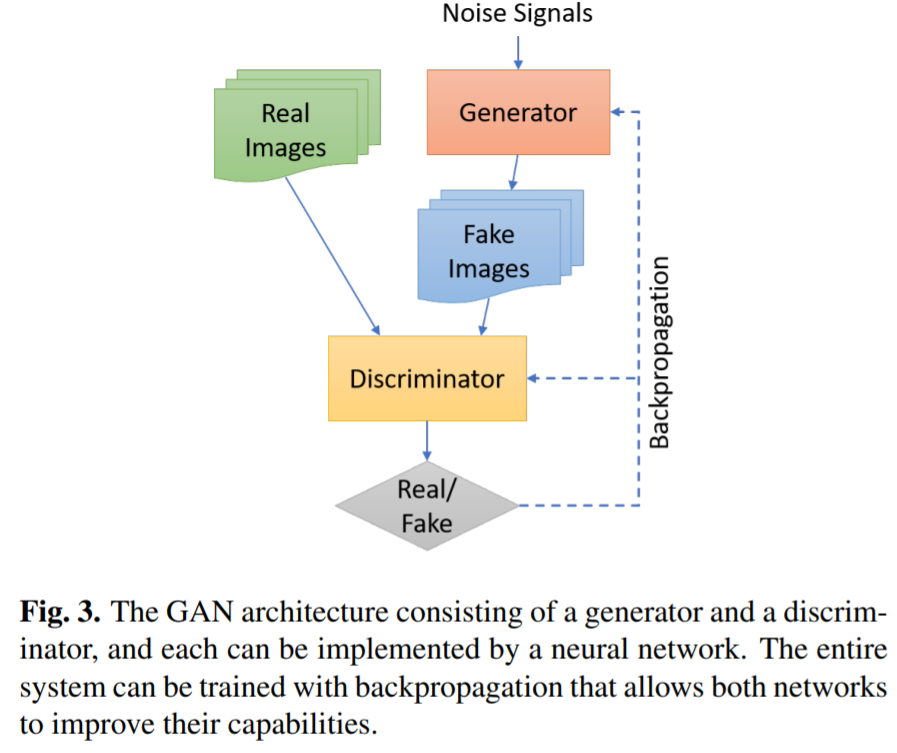
\includegraphics[width=0.90\textwidth]{img/ch3m9.png} 
\caption{ Thanh Thi Nguyen 等人 \cite{https://doi.org/10.48550/arxiv.1909.11573} GAN}
\label{Test}
\end{figure}

\begin{figure}[htb]
\centering 
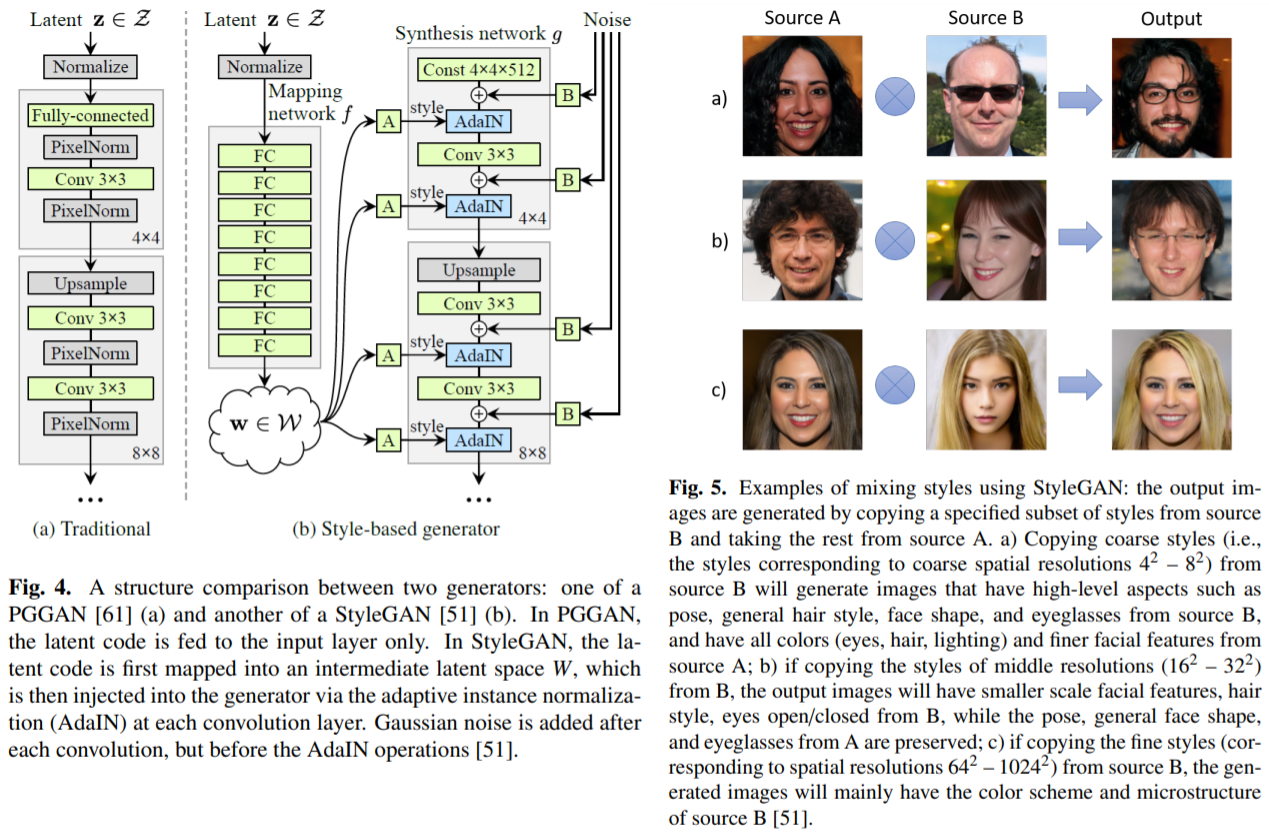
\includegraphics[width=1.05\textwidth]{img/ch3m11.png} 
\caption{ Thanh Thi Nguyen 等人 \cite{https://doi.org/10.48550/arxiv.1909.11573} PGGAN 和 StyleGAN}
\label{Test}
\end{figure}

另外 Nataraj L 等人 \cite{nataraj2019detecting}则是发现,生成对抗网络 (GAN) 的出现带来了全新的方式来转换和操纵数位图像中的像素,而基于 GAN 的技术,如图像到图像的转换、DeepFakes 和其他自动化方法在创建假图像方面变得越来越流行。在该研究中,研究者们提出了一种结合共现矩阵和深度学习来检测 GAN 生成的假图像的新方法,也就是在像素域中的三个颜色通道上提取共现矩阵,并使用深度卷积神经网络 (CNN) 框架训练模型。基于未配对的图像到图像转换(cycleGAN )和面部属性/表情(StarGAN )的两个多样化且具有挑战性的 GAN 数据集包含超过 56,000 张图像的实验结果表明,该研究的方法很有前景,并取得了超过两个数据集中的分类准确率为 99\%。此外,当在一个数据集上训练并在另一个数据集上进行测试时,此研究的方法也可以很好地泛化并取得良好的结果。

同时 Li H 等人 \cite{li2020identification},则借助强大的深度网络架构,例如生成对抗网络,人们可以轻松生成逼真的图像。尽管生成的图像并非专门用于欺骗人类或欺骗生物特征认证系统,但研究界和公共媒体对这些图像引起的安全问题表示了极大的关注。该研究解决了识别深度网络生成 (DNG) 图像的问题,考虑到相机成像和DNG图像生成之间的差异,研究者分析了不同颜色分量的DNG图像和真实图像之间的差异。其研究观察到 DNG 图像在色度分量中与真实图像更容易区分,尤其是在残差域中。基于这些观察,研究者们提出了一个特征集来捕获用于识别 DNG 图像的彩色图像统计信息。此外,研究者评估了几种检测情况,包括训练测试数据在图像源或生成模型中匹配或不匹配,以及仅使用真实图像进行检测。大量实验结果表明,该方法可以准确识别 DNG 图像,并且在训练和测试数据不匹配时优于现有方法。此外,当 GAN 模型未知时,研究者的方法也通过仅使用真实图像进行训练,实现了一类分类的良好性能。

而在图像的预处理上,Xuan X 等人 \cite{xuan2019generalization} 也发现最近 GAN 生成的人脸图像越来越逼真,质量越来越高,甚至人眼也很难检测到,另一方面,取证社区不断开发检测这些生成的虚假图像的方法,并试图保证视觉内容的可信度。尽管研究人员已经开发了一些检测生成图像的方法,但很少有人探索取证模型泛化能力的重要问题。随着新型 GAN 的快速涌现,取证模型检测新型 GAN 图像的泛化能力绝对是一个必不可少的研究课题。在该研究中,研究者们探讨了这个问题,并建议使用预处理图像来训练取证 CNN 模型。通过对真实和虚假的训练图像应用相似的图像级预处理,取证模型被迫学习更多的内在特征来对生成的和真实的人脸图像进行分类。而其的实验结果也证明了所提方法的有效性。

另外 McCloskey S 等人 \cite{mccloskey2018detecting} 图像取证是一个越来越相关的问题,因为它可以潜在地解决在线虚假信息活动并减轻社交媒体的问题方面。鉴于其最近的成功,特别令人感兴趣的是由生成对抗网络 (GAN) 生成的图像的检测,例如 '深度伪造',其利用大型训练集和广泛的计算资源,最近的工作表明,可以训练 GAN 生成合成图像,这(在某些方面)与真实图像无法区分,研究者们分析了一个流行的 GAN 实现的生成网络的结构,并表明该网络对颜色的处理在两个方面与真实相机明显不同。该研究进一步表明,这两个线索可用于区分 GAN 生成的图像和相机图像,证明了 GAN 图像和用于训练 GAN 的真实相机图像之间的有效区分。

另一方面在 GAN 的指纹上,Marra F 等人 \cite{marra2019gans} 则认为在过去的几年里,生成对抗网络(GAN)在计算机视觉和相关领域的许多应用中显示出巨大的潜力,以目前的发展速度,可以肯定的是,GAN 很快就能生成与真实图像和视频几乎无法区分的高质量图像和视频。不幸的是,真实的 GAN 生成的图像对安全构成了严重威胁,首先可能出现大量虚假多媒体,因此迫切需要多媒体取证对策。在该项工作中,研究者们展示了每个 GAN 在其生成的图像中留下其特定的指纹,就像现实世界的相机用它们的照片响应非均匀模式的痕迹标记所获取的图像一样。几种流行的 GAN 的源识别实验表明,这种指纹代表了类似于法医分析的宝贵资产。与此同时 Yu N 等人 \cite{yu2019attributing} 也认为生成对抗网络 (GAN) 的最新进展表明,在生成逼真的图像方面取得了越来越大的成功,但 GAN 也对视觉取证和模型归因提出了挑战。该研究提出了学习 GAN 指纹对图像属性的第一项研究,并使用它们将图像分类为真实图像或 GAN 生成的图像,而对于 GAN 生成的图像,研究者进一步识别它们的来源,其研究的实验表明(1)GAN 带有不同的模型指纹,并在其生成的图像中留下稳定的指纹,从而支持图像属性;(2) GAN 训练中即使是微小的差异也会导致不同的指纹,从而实现细粒度的模型认证;(3) 指纹在不同的图像频率和补丁上持续存在,并且不受 GAN 伪影的影响; (4) 指纹微调对五种对抗性图像扰动有效免疫;(5) 比较还表明,研究者的学习的指纹在各种设置中始终优于几个基线。

最后 Wang R 等人 \cite{wang1909fakespotter} 提出了一种名为 FakeSpotter 的新方法,该方法基于监视神经元行为来发现 AI 合成的假脸,对神经元覆盖和交互的研究已经成功地表明,它们可以作为深度学习系统的测试标准,尤其是在暴露于对抗性攻击的情况下。在这里,研究者们推测监控神经元行为也可以作为检测假脸的资产,因为逐层神经元激活模式可能会捕获对假人检测器很重要的更细微的特征。检测用最先进的 GAN 合成的四种假人脸并避免四种扰动攻击的实验结果表明了该研究方法的有效性和鲁棒性。

\begin{figure}[htb]
\centering 
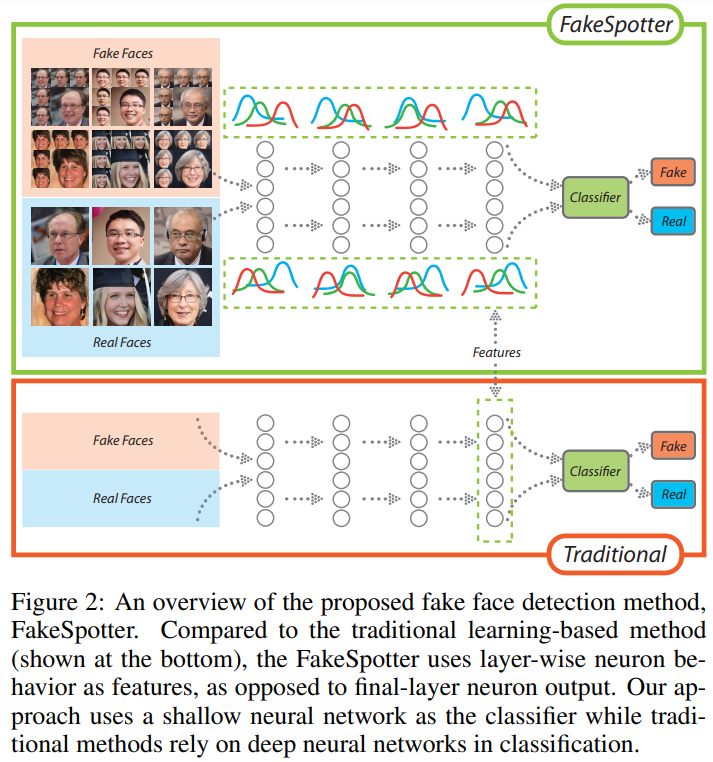
\includegraphics[width=0.90\textwidth]{img/ch3m10.png} 
\caption{ Wang R 等人 \cite{wang1909fakespotter} 运用神经元覆盖的方案来找出伪造出来的人脸}
\label{Test}
\end{figure}


\section{数据驱动的深度学习之检测手段}

由 Thanh Thi Nguyen 等人 \cite{https://doi.org/10.48550/arxiv.1909.11573} 与 Li XR 等人近期来的汇整工作\cite{2021496},图片的深度学习之检测手段与影像的深度学习之检测手段皆为数据驱动的深度学习,而所谓的数据驱动深度学习,其选择器都为深部结构,而特征是经过训练形成,而不是手工,大致上可将数据驱动的主动深度学习分成根据元学习下的主动深度学习、根据强化学习下的主动深度学习、根据不确定性学习下的主动深度学习、基于数据增强下的主动深度学习。

\begin{figure}[htb]
\centering 
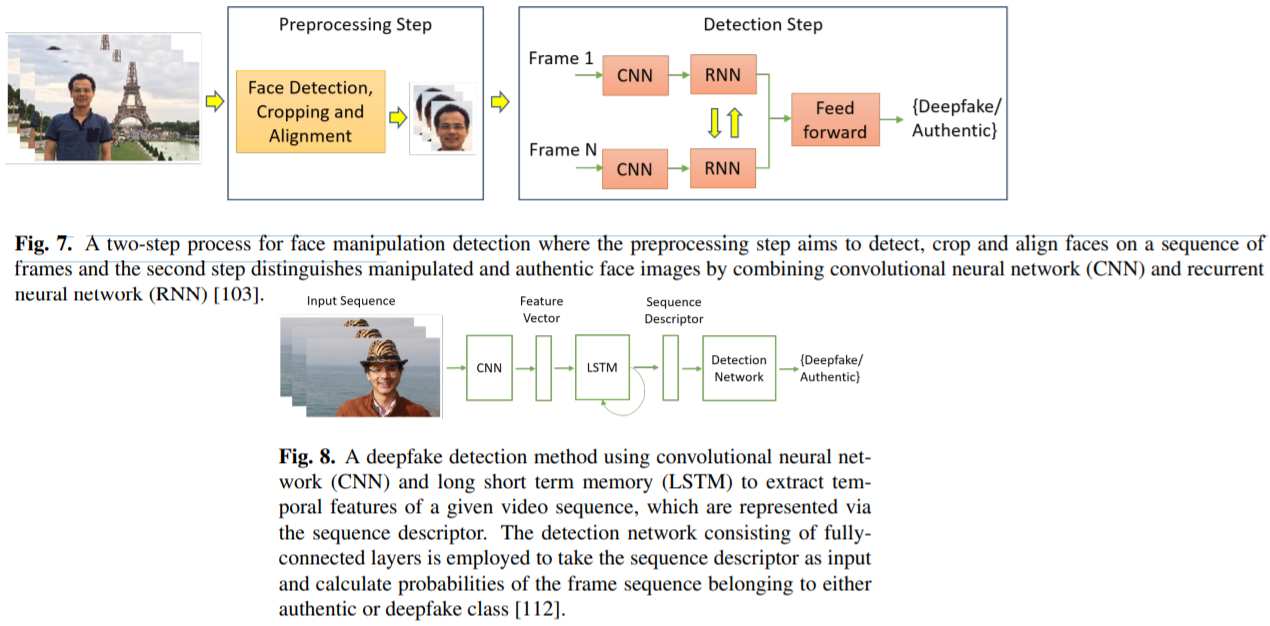
\includegraphics[width=1.05\textwidth]{img/ch3m12.png} 
\caption{ Thanh Thi Nguyen 等人 \cite{https://doi.org/10.48550/arxiv.1909.11573} 影像和图片}
\label{Test}
\end{figure}

而在深度伪造的发展下,其算法的规模与对应的数据量都相较过去有显著的增加,而且有不断成长的趋势,在此则分为图片处理与影像处理两大分类,前者的原理是将影片的处理成一帧帧的图像,而后对每帧的图像进行伪造检测处理,另外后者则是影像类,根据循环神经网路去对整个影片来做伪造检测。由下Thanh Thi Nguyen 等人 \cite{https://doi.org/10.48550/arxiv.1909.11573} 所做的工作总结,可以看到第一种是图像用于人脸操作检测的两步过程,其中预处理步骤旨在检测、裁剪和对齐一系列帧上的人脸,第二步通过结合卷积神经网络 (CNN) 和循环神经网络 (RNN) 来区分经过操作的和真实的人脸图像 )。另一种使用卷积神经网络 (CNN) 和长短期记忆 (LSTM) 提取给定视频序列的时间特征的深度伪造检测方法,这些时间特征通过序列描述符表示。由全连接层组成的检测网络用于将序列描述符作为输入,并计算帧序列属于真实类或 deepfake 类的概率。而后续图片的深度学习之检测手段与影像的深度学习之检测手段的细节则在后两节进行说明。


\section{图片的深度学习之检测手段}

此节讲述图片的深度学习之检测手段,Afchar D 等人 \cite{afchar2018mesonet} 提出了一種自動有效地檢測視頻中的人臉篡改的方法,特別關注最近用於生成超逼真偽造視頻的兩種技術:Deepfake 和 Face2Face,由於壓縮會嚴重降低數據質量,傳統的圖像取證技術通常不太適合視頻。因此,該研究采用深度學習方法並提出了兩個網絡,兩者都具有較少的層數,以專注於圖像的細觀特性。該研究在現有數據集和研究者從在線視頻構成的數據集上評估這些快速網絡。最後測試證明了非常成功的檢測率,Deepfake 的檢測率超過 98\%,Face2Face 的檢測率超過 95\%。

Rossler A 等人 \cite{rossler2019faceforensics++} 认为合成图像生成和处理的快速进展现在已经到了引发对社会影响的重大担忧的地步。充其量,这会导致对数字内容失去信任,但可能会通过传播虚假信息或虚假新闻而造成进一步的伤害,该研究研究了最先进的图像处理的真实性,以及自动或人工检测它们的难度,而为了标准化检测方法的评估,研究者提出了面部操作检测的自动化基准。特别是,该基准基于 DeepFakes、Face2Face、FaceSwap 和 NeuralTextures 作为随机压缩级别和大小的面部操作的突出代表。该基准是公开的,包含一个隐藏的测试集以及一个包含超过 180 万张操纵图像的数据库,而且该数据集相对于可比较的、公开可用的伪造数据集大一个数量级。基于这些数据,研究者们对数据驱动的伪造检测器进行了彻底的分析。其研究表明,即使在存在强压缩的情况下,使用额外的特定领域知识也可以将伪造检测提高到前所未有的准确性,并且明显优于人类观察者,其前者运用 Chollet F 等人 \cite{chollet2017xception} 的 Xception 架构进行对影像每一帧跟人类脸部进行分别训练,其训练结果好于全帧的模型训练结果。当中所谓 Xception 架构则是将卷积神经网络中的 Inception 模块解释为介于常规卷积和深度可分离卷积操作(深度卷积后跟点卷积)之间的中间步骤,从这个角度来看,深度可分离卷积可以理解为具有最大数量的塔的 Inception 模块,这一观察使研究者提出了一种受 Inception 启发的新型深度卷积神经网络架构,其中 Inception 模块已被深度可分离卷积取代。其研究表明,这种被称为 Xception 的架构在 ImageNet 数据集(Inception V3 的设计目标)上略微优于 Inception V3,并且在包含 3.5 亿张图像和 17,000 个类别的更大图像分类数据集上显著优于 Inception V3。由于 Xception 架构与 Inception V3 具有相同数量的参数,因此性能提升不是由于容量增加,而是更有效地使用模型参数。

而运用找出人脸的关键部位来提升模型训练成果,则有 Songsri-in K 等人 \cite{songsri2019complement} 在其研究进行验证,其研究是提出了第一个严格的人脸取证定位数据集,该数据集由真实的、生成的和经过处理的人脸图像组成。特别是,原始部分包含来自 CelebA 和 FFHQ 数据集的人脸图像。假图像是由各种 GANs 方法生成的,即 DCGANs、LSGANs、BEGANs、WGAN-GP、ProGANs 和 StyleGANs。最后,编辑的子集是基于自由形式掩码从 StarGAN 和 SEFCGAN 生成的。该数据集总共包含大约 130 万张用相应的二进制掩码标记的面部图像。基于所提出的数据集,研究者们证明了在输入图像之外显式添加面部标志信息可以提高性能。此外,该研究提出的方法由两个分支组成,可以连贯地预测人脸取证检测和定位,以优于以前在新提出的数据集以及 faceforecsic++ 数据集上的最新技术,尤其是在低质量视频上。而 Nguyen HH 等人 \cite{nguyen2019capsule} 认为媒体生成技术的最新进展使攻击者更容易创建伪造的图像和视频,其最先进的方法可以实时创建从社交网络获得的单个视频的伪造版本。尽管已经开发了许多用于检测伪造图像和视频的方法,但它们通常针对某些领域,并且随着新型攻击的出现很快就过时了。该研究介绍的方法使用胶囊网络来检测各种欺骗,从使用打印图像或录制视频的重放攻击到使用深度卷积神经网络的计算机生成视频,它将胶囊网络的应用扩展到解决逆图形问题的初衷之外,该研究更重要的一点在运用了 Simonyan K 等人 \cite{simonyan2014very} 所做的 VGG-19,其主要贡献是使用具有非常小的 (3x3) 卷积滤波器的架构对深度增加的网络进行了全面评估,这表明通过将深度提升到 16-19 个权重层可以实现对现有技术配置的显著改进,这些发现是研究者们提交 2014 年 ImageNet 挑战赛的基础,该研究团队分别获得了定位和分类轨道的第一和第二名。该研究还表明,其表示可以很好地推广到其他数据集,并在这些数据集上取得了最先进的结果。

Mo H 等人 \cite{mo2018fake} 则发现生成对抗网络 (GAN) 是一种突出的生成模型,广泛用于各种应用,最近的研究表明,基于这种新颖的模型可以获得具有高视觉质量的假人脸图像。如果这些假脸被滥用于图像篡改,将导致一些潜在的道德、伦理和法律问题。因此,在该研究的研究者们首先提出了一种基于卷积神经网络(CNN)的方法来识别当前最佳方法生成的假人脸图像,并提供实验证据表明该方法可以达到令人满意的结果,平均准确率超过 99.4 \%。此外,研究者们提供了对所提出的 CNN 架构的一些变体进行评估的比较结果,包括高通滤波器、层组数和激活函数,以进一步验证我们方法的合理性。

\begin{figure}[htb]
\centering 
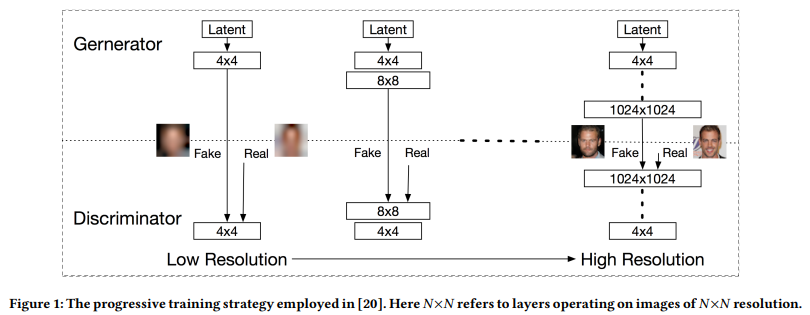
\includegraphics[width=1.05\textwidth]{img/ch3m13.png} 
\caption{Mo H 等人 \cite{mo2018fake}}
\label{Test}
\end{figure}

Durall R 等人 \cite{durall2019unmasking} 运用离散傅立叶变换的方法来进行特征学习 就此提出了一种检测此类假人脸图像的简单方法,也就是检测所谓的 DeepFakes,该研究的方法基于经典的频域分析,然后是基本分类器。与需要输入大量标记数据的先前系统相比,我们的方法仅使用少量带注释的训练样本就显示出非常好的结果,甚至在完全无监督的情况下也取得了很好的准确性。对于高分辨率人脸图像的评估,研究者将几个真实和虚假人脸的公共数据集组合成一个新的基准:Faces-HQ。鉴于如此高分辨率的图像,当该研究的方法在少至 20 个带注释的样本上进行训练时,其方法达到了 100\% 的完美分类准确率。在第二个实验中,在 CelebA 数据集的中等分辨率图像的评估中,其方法在有监督的情况下达到了 100\% 的准确率,在无监督的情况下达到了 96\%。最后,评估 FaceForensics++ 数据集的低分辨率视频序列,该研究的方法检测操纵影片的准确率达到 91\%。Ding X 等人 \cite{ding2020swapped} 在这项研究中,使用深度迁移学习进行人脸交换检测,也就是运用 Resnet18 进行改良,其结果显示出大于 96\% 的真阳性率,并且误报率非常低。与仅提供检测准确性的现有方法不同,该研究还为每个预测提供不确定性,这对于信任此类检测系统的部署至关重要。此外,研究者们提供了与人类受试者的比较。为了捕捉人类识别性能,此研究建立了一个网站来收集人类受试者图像的成对比较。基于这些比较,研究者们推断出从被认为最真实的图像到被认为最假的图像的共识排名,总体而言,结果显示了该研究的方法有效性。作为这项研究的一部分,研究者们创建了一个新的数据集。

而 Cozzolino D 等人 \cite{cozzolino2018forensictransfer} 引入了取证转移(FT)。研究者们设计了一种基于学习的取证检测器,它可以很好地适应新领域,即新颖的操作方法,并且可以处理在训练期间只有少数假样本可用的场景。为此,研究者学习了一种基于新型自动编码器架构的取证嵌入,该架构可用于区分真假图像,其学习嵌入充当异常检测器的一种形式;即,如果从不可见的方法处理的图像与真实图像集群足够远,则该图像将被检测为假图像。与之前的工作相比,FT 显示出可迁移性的显著改进,该研究在一系列关于尖端基准的实验中证明了这一点。例如,在未见过的例子上,研究者们的准确率高达 85\%,而只有少数可见的例子,该研究性能已经达到了 95\% 左右。

就 Cozzolino D 等人 \cite{cozzolino2018forensictransfer} 的研究成果上,其 Nguyen HH 等人 \cite{nguyen2019multi} 认为检测被操纵的图像和视频是数字媒体取证中的一个重要课题,大多数检测方法使用二进制分类来确定查询被操纵的概率,另一个重要主题是定位被操纵区域(即执行分割),这主要是由三种常用攻击创建的:删除、复制移动和拼接。研究者们设计了一个卷积神经网络,它使用多任务学习方法来同时检测被操纵的图像和视频,并为每个查询定位被操纵的区域,其通过执行一项任务获得的信息与另一项任务共享,从而提高两项任务的性能。另外使用半监督学习方法来提高网络的可生成性,该网络包括一个编码器和一个 Y 形解码器。编码特征的激活用于二进制分类,其解码器一个分支的输出用于分割操作区域,而另一个分支的输出用于重构输入,这有助于提高整体性能。使用 FaceForensics 和 FaceForensics++ 数据库的实验证明了该网络对面部重演攻击和面部交换攻击的有效性,以及它处理先前看到的攻击的不匹配条件的能力。此外,仅使用少量数据进行微调使网络能够处理看不见的攻击。

Hsu CC 等人 \cite{hsu2018learning} 开发一种深度伪造鉴别器(DeepFD)来有效地检测计算机生成的图像,其直接学习二元分类器相对比较棘手,因为很难找到共同的判别特征来判断不同 GAN 生成的假图像。为了解决这个缺点,研究者采用对比损失来寻找由不同 GAN 生成的合成图像的典型特征,然后连接一个分类器来检测这些计算机生成的图像,实验结果表明,所提出的 DeepFD 成功检测到由几个最先进的 GAN 生成的 94.7\% 的假图像。同样也是 Hsu CC 等人 \cite{hsu2020deep} 提出了一种基于深度学习的方法,通过使用对比损失来检测假图像。首先,采用几种最先进的 GAN 来生成假-真图像对。接下来,将简化的 DenseNet 发展为双流网络结构,以允许成对信息作为输入。然后,使用成对学习来训练所提出的常见假特征网络,以区分假图像和真实图像之间的特征。最后,将分类层连接到所提出的常见假特征网络,以检测输入图像是假的还是真的,其实验结果表明,所提出的方法明显优于其他最先进的假图像检测器。

另外 Dang LM 等人 \cite{dang2018deep} 提出了一种定制的卷积神经网络,即 CGFace,它是专门为计算机生成的人脸检测任务而设计的,通过自定义卷积层的数量,因此在检测计算机生成的人脸图像方面表现良好。之后,通过从 CGFace 层中提取特征并使用它们来训练 AdaBoost 和 eXtreme Gradient Boosting (XGB) 来改变 CGFace 的层结构以适应不平衡数据问题,从而创建了一个不平衡框架 (IF-CGFace)。接下来,研究者们将解释基于最先进的 PCGAN 和 BEGAN 模型生成大型计算机生成数据集的过程。而随后的进行了各种实验也表明所提出的具有增强输入的模型产生了 98\% 的最高精度。最后,研究者们通过将所提出的 CNN 架构应用于其他 GAN 研究生成的图像来提供比较结果。

Bayar B 等人 \cite{bayar2016deep} 提出了一种通用的取证方法来使用深度学习执行操作检测。具体来说,研究者们提出了一种新的卷积网络架构,能够直接从训练数据中自动学习操作检测特征,而在目前的形式中,卷积神经网络将学习捕捉图像内容的特征,而不是操作检测特征。为了克服这个问题,该研究开发了一种新形式的卷积层,专门用于抑制图像的内容并自适应地学习操作检测特征,通过一系列实验,其研究证明了研究者们提出的方法可以自动学习如何检测多个图像操作,而不依赖于预先选择的特征或任何预处理。这些实验的结果表明,该研究提出的方法可以自动检测几种不同的操作,平均准确率为 99.10\%。

Li X 等人 \cite{li2020fighting} 提出了一种新颖的 Patch\&Pair 卷积神经网络 (PPCNN) 来区分 Deepfake 视频或图像与真实视频或图像,其通过对公共数据集的综合评估,研究者证明其研究的模型比现有的检测方法表现更好,并表现出更好的泛化性。

\begin{figure}[htb]
\centering 
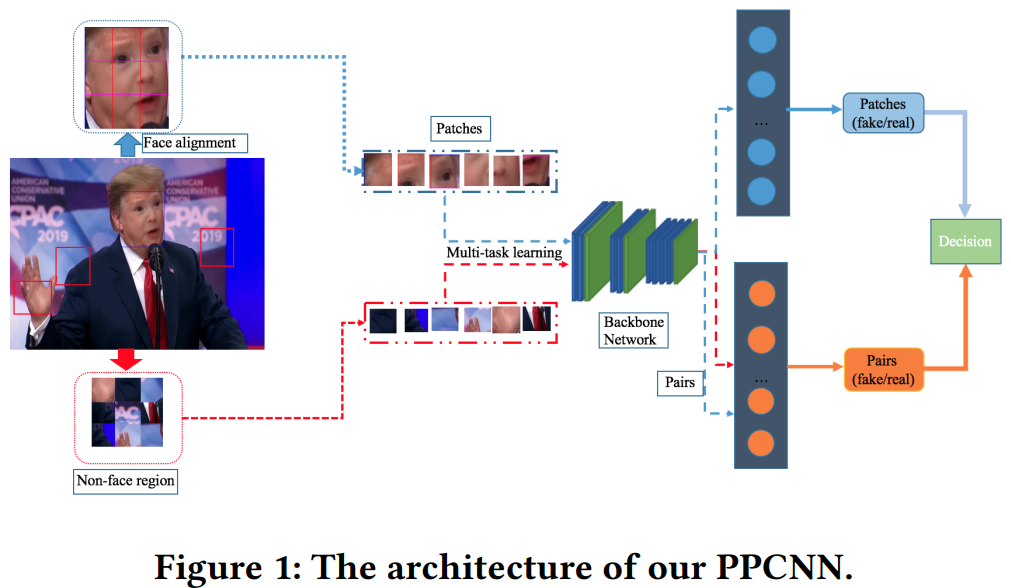
\includegraphics[width=1.05\textwidth]{img/ch3m14.png} 
\caption{Li X 等人 \cite{li2020fighting} 提出了一种新颖的 Patch\&Pair 卷积神经网络 (PPCNN)}
\label{Test}
\end{figure}

Rahmouni N 等人 \cite{rahmouni2017distinguishing} 提出了一种深度学习方法,用于将计算机生成的图形与真实的摄影图像区分开来。所提出的方法使用带有自定义池化层的卷积神经网络 (CNN) 来优化当前性能最佳的算法特征提取方案,来计算和聚合类概率的局部估计以预测整个图片的标签,研究者评估了我们在最近的照片般逼真的计算机图形方面的工作,并表明它在局部和完整图像分类方面都优于最先进的方法。

Dang H 等人  \cite{dang2020detection} 建议利用注意力机制来处理和改进分类任务的特征图,而不是简单地使用多任务学习来同时检测操纵图像和预测操纵掩码(区域),其学习到的注意力图突出显示信息区域以进一步改进二元分类(真人脸与假人脸),并可视化操作区域,为了使研究者能够研究操纵的面部检测和定位,该研究收集了一个包含多种类型的面部伪造的大型数据库。同时使用这个数据集的过程中,研究者对数据驱动的假人脸检测进行了彻底的分析,成果展示了注意力机制的使用改进了面部伪造检测和操纵区域定位。

Brockschmidt J 等人 \cite{brockschmidt2019generality} 研究了最先进的面部伪造检测架构的泛化能力,其研究者首先提出两个通用性标准:可靠地检测多种欺骗技术和可靠地检测看不见的欺骗技术,随后设计实验来衡量给定架构如何根据这些标准执行。研究者的分析侧重于两种最先进的面部伪造检测架构,MesoNet 和 XceptionNet,它们都是卷积神经网络 (CNN),而实验使用来自六种最先进的面部伪造技术的样本:Deepfakes、Face2Face、FaceSwap、GANnotation、ICface 和 X2Face。研究者发现 MesoNet 和 XceptionNet 显示出泛化到多种欺骗技术的潜力,但在准确性上略有权衡,并且在很大程度上无法对抗看不见的技术。最后将这些结果松散地推断为类似的 CNN 架构,并强调需要更好的架构来应对普遍性的挑战。 Sohrawardi SJ 等人 \cite{sohrawardi2019poster}  研究者们提出了一个系统,该系统将强大而有效地使用户能够确定在线发布的影片是否是 deepfake,该研究从记者的角度处理问题,并努力开发一种工具以无缝融入他们的工作流程,结果表明对内部数据集和不匹配数据集的准确检测。综上所述,若是在影像中每一帧帧去检测伪造的方式,在一整部影像伪造地方过少,很有可能没有办法检测的到。那图片的检测手段方式很可能会有严峻的挑战与不理想得结果。

\section{影像的深度学习之检测手段}

此节讲述影像的深度学习之检测手段,Agarwal S 等人 \cite{agarwal2019protecting} 发现从每个个体来看,运用针对人类脸部的追踪,跟面对人体的头部移动抽取特定动作,其脸部的肌肉变化的可以做为动作单元,同时运用皮尔森系数找出对每个特征间的关联,最后根据此来建立一个 SVM 分类伪造出来的影像。尽管在视觉上并不明显,但这些相关性经常被深度伪造视频的创建方式所破坏,因此可以用于身份验证。
另外 Amerini I \cite{amerini2019deepfake} 在这项工作中,给出了一种能够区分假视频序列和原始视频序列的新取证技术; 与采用单个视频帧的其他最先进的方法不同,研究者们建议采用光流场来利用可能的帧间差异。然后将这样的线索用作 CNN 分类器要学习的特征,其分类器为 VGG16,最后在 FaceForensics++ 数据集上获得的初步结果突出了非常有前景的性能。

Güera D 等人\cite{guera2018deepfake} 提出了一种时间感知管道来自动检测 deepfake 视频。研究者的系统使用卷积神经网络 (CNN) 来提取帧级特征,然后使用这些特征来训练循环神经网络 (RNN),该网络学习对视频是否受到操纵进行分类。同时研究者针对从多个视频网站收集的大量 deepfake 视频评估该研究的方法,最后展示了该研究的系统如何在使用简单架构的同时在这项任务中取得有竞争力的结果。

其框架分成了两个不同阶段的分析器,一个为 CNN 去找出每一个帧内的特征,然后放进所需要的序列,最后交给 LSTM 进行分析,回传一个机率的判断结果。另外在 Li XR 等人近期来的汇整工作\cite{2021496} 中也有详细说明其循环神经网路和卷积的判断机制。

\begin{figure}[htb]
\centering 
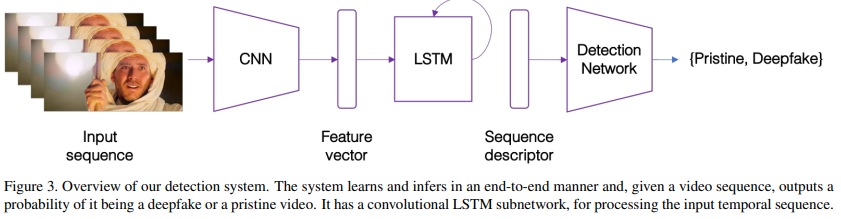
\includegraphics[width=1.05\textwidth]{img/ch3m15.png} 
\caption{Güera D \cite{guera2018deepfake} 架構}
\label{Test}
\end{figure}

\begin{figure}[htb]
\centering 
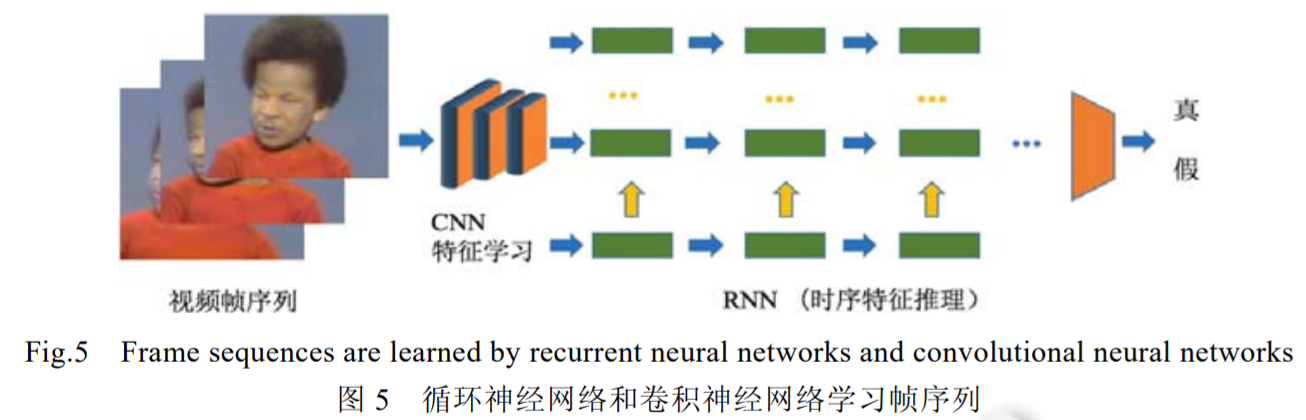
\includegraphics[width=1.05\textwidth]{img/ch3m16.png} 
\caption{Li XR 汇整工作\cite{2021496} 中详细说明其循环神经网路和卷积的判断机制}
\label{Test}
\end{figure}

另外 Sabir E 等人 \cite{sabir2019recurrent} 通过广泛的实验提取了将这些模型的变化与特定领域的面部预处理技术相结合的最佳策略,以在公开的基于视频的面部操作基准上获得最先进的性能。具体来说,该研究尝试检测视频流中的 Deepfake、Face2Face 和 FaceSwap 篡改人脸,其评估是在最近推出的 FaceForensics++ 数据集上进行的,将之前最先进的准确率提高了 4.55\%,其关键的地方在采用了双向时序网络和人脸对齐并用的方式去判断伪造出来的生成结果,当中最好的部分是的人脸对齐跟 Bidrectional-recurrent-denset 的伪造检测上。由上述可知,虽然影像的深度学习等之检测手段,泛化性高,同时可以找到影片中少量的篡改,但是在面对压缩过后的影像、光影变化时的伪造检测却很无力。

\section{人类语音伪造检测手段}

随着深度伪造在人类语音技术合成的发展,此类工作也受到研究者的关注。 Todisco M 等人 \cite{todisco2016new} 发现近年来,开发新的对策以保护自动说话人验证免受欺骗的努力已经加强,其 ASVspoof 2015 计划表明,检测欺骗攻击的潜力很大,但检测以前无法预见的欺骗攻击仍然具有挑战性,该研究认为,从研究特征而不是分类器中可以获得更多收益,并介绍了一种基于恒定 Q 变换的欺骗检测新特征,这是一种在音乐研究中流行的受感知启发的时频分析工具。使用标准 ASVspoof 2015 数据库获得的实验结果表明,当与基于标准高斯混合模型的分类器结合使用时,所提出的恒定 Q 倒谱系数 (CQCC) 的性能明显优于所有先前报告的结果,特别是,对于未知欺骗攻击子集(未使用匹配的训练数据)的攻击为 0.46\%,相对于先前报告的最佳结果提高了 72\%。

同时 Wu Z 等人 \cite{wu2012study} 首先展示了评估当前最先进的说话人验证系统的脆弱性的新结果:具有联合因子分析 (GMM-JFA) 和概率线性判别分析 (PLDA) 系统的高斯混合模型,以防止欺骗攻击。而所谓的欺骗攻击则是通过两种语音转换技术模拟:基于高斯混合模型的转换和基于单元选择的转换。为了降低由欺骗攻击引起的错误接受率,研究者提出了一种用于说话人验证系统的通用反欺骗攻击框架,其中采用转换后的语音检测器作为说话人验证系统接受决策的后处理模块,其检测器决定接受的声明是人类语音还是转换后的语音。 NIST SRE 2006 语料库中的核心任务子集用于评估说话人验证系统的脆弱性和转换后的语音检测器的性能。其研究结果表明,两种转换技术都可以提高 GMM-JFA 和 PLDA 系统的误认率,而转换后的语音检测器可以将 GMM-JFA 和 PLDA 的误认率从 31.54\% 和 41.25\% 降低到 1.64\% 和 1.71\%基于单元选择的转换语音系统。同样地,Wu Z 等人 \cite{wu2012detecting} 建议使用从相位谱中获得的特征来检测转换后的语音。这些特征在转换后的语音检测器的三种不同训练情况下进行测试: a) 只有基于高斯混合模型 (GMM) 的转换后的语音数据可用; b) 只有基于单元选择的转换语音数据可用; c) 没有转换后的语音数据可用于训练转换后的语音模型。而在美国国家标准与技术研究院 (NIST) 2006 说话人识别评估 (SRE) 语料库上进行的实验表明,从相位谱派生的特征的性能大大优于梅尔频率倒谱系数 (MFCC):即使没有经过转换的语音进行训练,等错误率 (EER) 从 MFCC 的 20.20\% 降低到 2.35\%。

Das RK 等人 \cite{das2019long} 考虑了基于远程声学特征的新对策,这些对策在许多方面都是独一无二的,因为它们是使用倍频程功率谱和子带得出的,而不是常用的线性功率谱,在挑战后研究中,研究者进一步研究了使用深度特征来增强真实和欺骗性语音之间的区分能力。而该研究在从远程声学和深度特征的角度总结了欺骗检测的发现,并从不同类型的欺骗攻击的性质和系统开发进行了综合分析。

Zeinali H 等人 \cite{zeinali2019detecting} 的研究介绍了布尔诺理工大学 (BUT) 和 Omilia 共同努力的系统描述 — ASVSpoof2019 Spoofing and Countermeasures Challenge 的对话智能,其物理访问(PA)的主要提交是两个 VGG 网络的融合,并在单通道和双通道特征上进行了训练。对于逻辑访问 (LA),研究者的主要系统是 VGG 和最近引入的 SincNet 架构的融合,其 PA 上的结果表明,所提出的网络在所有条件下都产生了非常有竞争力的性能,并且与官方基线相比实现了 86\% 的相对改进。另一方面,LA 上的结果表明,尽管所提出的架构和训练策略在某些欺骗攻击上表现得非常好,但它无法推广到在训练期间看不见的某些攻击下。另外前者运用了 CQT 特征和功率谱图进行学习,而所谓的 CQT  则是 Schörkhuber C 等人 \cite{schorkhuber2010constant} 所提出了一种计算时域信号恒定 Q 变换 (CQT) 的高效计算方法。 CQT 指的是一种时频表示,其中频率区间是几何间隔的,并且所有区间的 Q 因子(中心频率与带宽的比率)相等,该研究提出了一种逆变换,它能够根据其 CQT 系数对原始信号进行合理质量(大约 55dB 信噪比)的重构。在这里,具有高 Q 因子的 CQT(相当于每倍频程 12-96 个 bin)特别令人感兴趣。所提出的方法在每倍频程的 bin 数量、应用的窗口函数和 Q 因子方面是灵活的,并且特别适用于音乐信号的分析。而提出方法的参考实现作为 Matlab 工具箱发布,该工具箱包括用户界面工具,可促进光谱数据可视化以及索引和使用 CQT 生成的数据结构。

Gomez-Alanis A 等人 \cite{gomez2019light} 这项工作的目的是开发一个单一的反欺骗系统,该系统可用于有效检测 ASVspoof 2019 挑战赛中考虑的所有类型的欺骗攻击:从文本到语音、语音转换和基于重放的攻击,而该研究为了实现这一点,研究者们建议使用轻卷积门控循环神经网络 (LC-GRNN) 作为深度特征提取器,以稳健地将语音信号表示为话语级嵌入,稍后由后端识别器使用,该识别器执行最终的真实/欺骗分类,这种新颖的架构结合了轻卷积层在帧级别提取判别特征的能力与基于门控循环单元的 RNN 学习后续深度特征的长期依赖关系的能力。所提出的系统已作为对 ASVspoof 2019 挑战赛的贡献而提出,与基线系统相比,结果显示出显著改进。此外,还在 ASVspoof 2015 和 2017 语料库上进行了实验,结果表明我们的提议明显优于最近提出的其他流行方法和其他类似的基于深度特征的系统。另外 Chen T 等人 \cite{chen2020generalization} 则由于最近语音合成和语音转换技术的突破,Audio Deepfakes,在技术上被称为逻辑访问语音欺骗技术,已经成为语音接口上越来越大的威胁。为了有效检测这些攻击对于包括自动说话人验证系统在内的许多语音应用程序至关重要,同时随着新型语音合成和语音转换技术的迅速出现,欺骗对策的泛化能力正成为越来越关键的挑战。该研究重点通过使用大余量余弦损失函数 (LMCL) 和在线频率掩蔽增强来强制神经网络学习更稳健的特征嵌入来克服这个问题,而研究者在 ASVspoof 2019 逻辑访问 (LA) 数据集上评估了拟议系统的性能。此外,研究者使用公开可用的噪声在 ASVspoof 2019 数据集的噪声版本上对其进行评估,以模拟更真实的场景,最后在通过电话通道逻辑重放的资料集副本上评估所提出的系统,以模拟呼叫中心场景中的欺骗攻击。研究者们的基线系统基于残差神经网络,并在 ASVspoof 2019 挑战期间的所有单系统提交中实现了 4.04\% 的最低等错误率 (EER),此外,该研究提出的额外改进将 EER 降低到 1.26\%。

\begin{figure}[htb]
\centering 
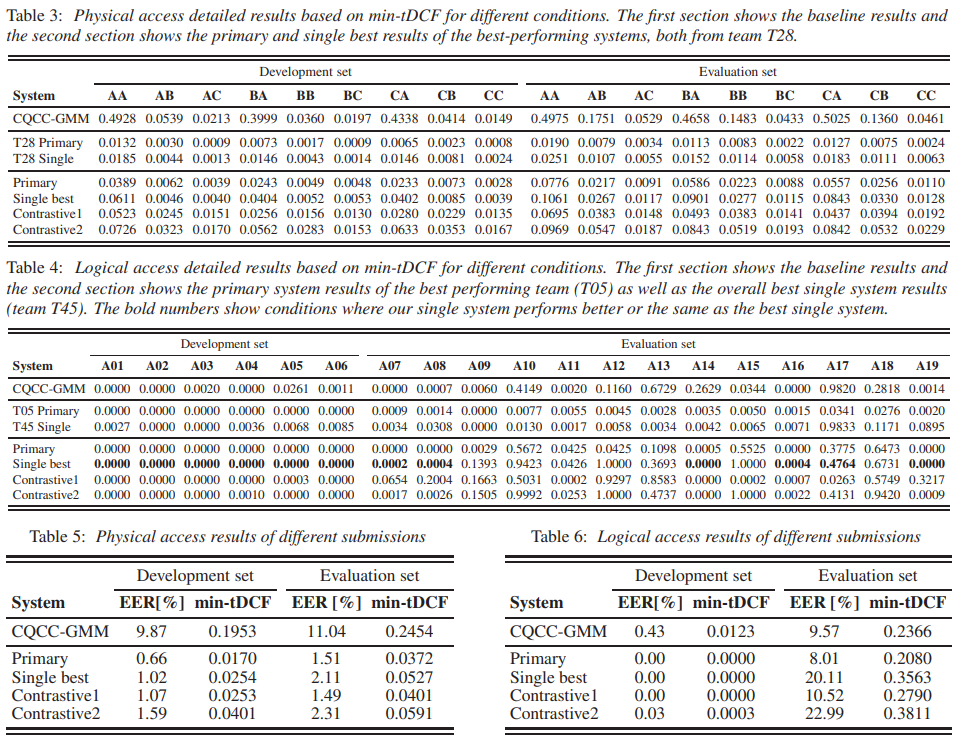
\includegraphics[width=1.05\textwidth]{img/ch3m17.png} 
\caption{Zeinali H 等人 \cite{zeinali2019detecting} }
\label{Test}
\end{figure}

\section{代表性检测技术整理与比较}

Li XR 等人近期来的汇整工作\cite{2021496},其针对各个检测的代表性的主流深度伪造的手段皆有整理,在此本作业根据其技术总结条列其特性、使用模型与相关研究者,使对应由 Thanh Thi Nguyen 等人 \cite{https://doi.org/10.48550/arxiv.1909.11573} 所整理的深度伪造检测工具表列,做一个互相呼应,而更重要的在于Li XR 等人总结出五大深度伪造检测方法的局限性跟在优势与劣势。

\begin{figure}[htb]
\centering 
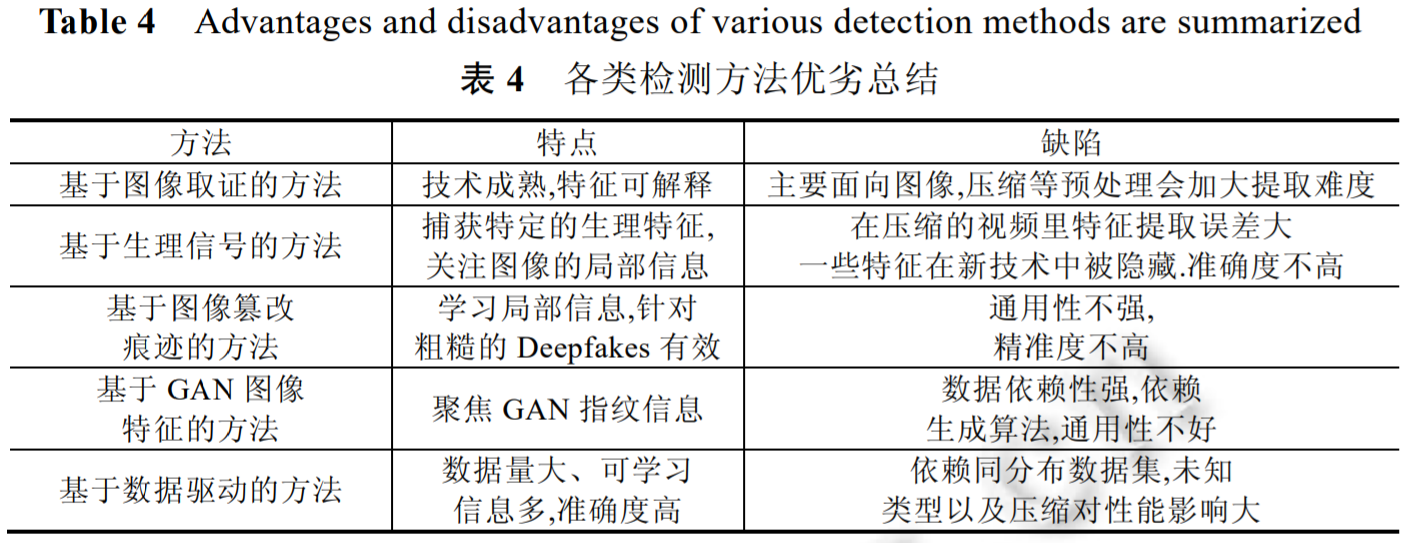
\includegraphics[width=1.05\textwidth]{img/ch3m18.png} 
\caption{Li XR 等人近期来的汇整工作\cite{2021496} ,其五大深度伪造检测方法的局限性跟在优势与劣势}
\label{Test}
\end{figure}

\begin{itemize}
\item [-] Fridrich J 等人 \cite{fridrich2012rich} 使用 SVM 模型,其特点为高通图像的隐写特征。
\item [-] Cozzolino D 等人 \cite{cozzolino2017recasting} 使用 CNN 模型,特色为残差特征的学习。
\item [-] Afchar D 等人 \cite{afchar2018mesonet} 使用 CNN ,特点是微观特征的学习。
\item [-] Rossler A 等人 \cite{rossler2019faceforensics++} 的 Xception 模型 ,其特色为对整帧的人脸区域学习。
\item [-] Nguyen HH 等人\cite{nguyen2019capsule} 使用模型为 CNN + 胶囊网络,而特色为 胶囊网络分类。
\item [-] Cozzolino, D 等人 \cite{cozzolino2018forensictransfer} 使用模型为 Autoencoder,而特色是用于分类和分割双任务。
\item [-] Nguyen HH 等人 \cite{nguyen2019multi} 使用模型为 Autoencoder ,其特色为分类和分割重建融合。
\item [-] Agarwal S 等人 \cite{agarwal2019protecting} ,其模型为 SVM ,而特色则为动作单元编码。
\item [-] Güera D 等人 \cite{guera2018deepfake} 使用了 CNN + RNN 的模型,而特点则是 图片的时序信息。
\item [-] Sabir E 等人 \cite{sabir2019recurrent} 使用模型为 CNN + Bi-LSTM,而特色为 图片的时序信息 。
\item [-] Zhou P 等人 \cite{zhou2017two} 使用 CNN + SVM 模型,并有人脸和隐写特征结合。
\item [-] Li Y 等人 \cite{li2018exposing} 使用 CNN 模型,特点为学习人脸边框篡改遗留痕迹。
\item [-] Matern F 等人 \cite{matern2019exploiting} 使用 Logistic Regression + MLP,其特色为学习篡改痕迹的细节缺失。
\item [-] Yang X 等人 \cite{yang2019exposing} 使用 SVM 模型,并针对头部姿态评估。
\item [-] Korshunova I 等人 \cite{korshunova2017fast} ,而模型方案则是 PCA + RNN 和 PCA + LDA,其特色为图像质量与声频校对
\item [-] Bayar B 等人 \cite{bayar2016deep}
\item [-] Dang H 等人 \cite{dang2020detection} 其使用模型为 CNN + Attention ,特色则是增加注意力机制。
\item [-] Chen T 等人 \cite{chen2020generalization} 使用模型则是 Deep Residual Network + Frequency Masking,而特点则是大边际距离损失函数。
\item [-] Gomez-Alanis A, 等人 \cite{gomez2019light} 使用模型为 LightCNN + RNN ,而特色为混合光卷积和门递归单元。
\item [-] Li R 等人 \cite{li2019anti} 模型则是 Butterfly Unit Multi-Task,特色为多特征融合与多任务学习。
\item [-] Zeinali H 等人 \cite{zeinali2019detecting} 而模型为 Light CNN 、VGG、SincNet,而特点则是多网络融合。
\end{itemize}












